\chapter{Especificación de requisitos}
\label{cap:especificacion-requisitos}

\section{Introducción}
En esta sección se describirá qué sistema vamos a construir y cómo lo vamos a hacer, 
con sus restricciones específicas. Esto se realizará especificando y describiendo
 los requisitos del sistema que vamos a desarrollar. 

\subsection{Propósito}
En este capítulo se pretende describir de forma clara y precisa las funciones, carasterísticas y restricciones
del sistema que se va a desarrollar. Estas definiciones servirán al equipo de desarrolo para
conocer las necesidades del sistema y a los usuarios finales. Además, este capítulo será será consultado como
base para el desarrollo de las funcionalidades descritas en la sección de implementación.

\subsection{Ámbito del Sistema}
El sistema que vamos a desarrollar es una aplicación multiplataforma llamada "Meloudy" que permitirá a los usuarios
aprender conceptos musicales de una forma amena, fácil y divertida. Esto se logrará mediante el método de gamificación,
utilizando un sistema de logros y de recompensas con la superación de los distintos ejercicios y actividades de distintos tipos que el usuario deberá completar.
Además, la aplicación llevará el progreso de los usuarios que les permitirá saber cómo van en su aprendizaje.

\subsection{Definiciones, Acrónimos y Abreviaturas}
A continuación se detallará el significado de algunos conceptos importantes para la comprensión del capítulo y de nuestro sistema.
\begin{itemize}
    \item \textbf{Requisito:} Es una condición o característica que debe cumplir el sistema para satisfacer una necesidad o cumplir una función.
    \item \textbf{Funcionalidad:} Descripción de lo que debe hacer el producto software.
    \item \textbf{Restricción:} Condición que limita la funcionalidad del sistema.
    \item \textbf{Interfaz de usuario:} Requisitos que describen los diseños de pantallas que utilizará el usuario para utilizar el software.
    \item \textbf{Usuario: }Persona que utilizará la aplicación para la intención final de esta.
    \item \textbf{Administrador: } Persona encargada del sistema software y del mantenimiento de este para su buen funcionamiento.
    \item \textbf{RF / RNF:} Requisito funcional / Requisito No Funcional.
\end{itemize}

\subsection{Referencias}
Este capítulo de Especificación de requisitos ha sido redactada consultando los documentos del estándar IEEE Recommended Practice for Software Requirements Specification ANSI/IEEE 830, 1998.

\subsection{Visión General del Documento}
La Especificación de Requisitos consta de tres partes bien diferenciadas:
\begin{itemize}
    \item \textbf{Introducción:} Proporciona una visión general sobre el apartado de Especificación de Requisitos sin profundizar en los requisitos como tal.
    \item \textbf{Descripción General:} Se describirá el sistema a construir para saber las funciones principales, los datos necesarios, las restricciones y otros aspectos que puedan afectar al desarrollo de la aplicación.
    \item \textbf{Requisitos Específicos:} Se profundiza en las necesidades del usuario definiendo los requisitos que debe tener nuestro sistema tras el desarrollo y la implementación de este.
\end{itemize}

\section{Descripción General}
A continuación, se procederá a describir la visión del sistema y los factores que afectan al producto de una forma general.

\subsection{Perspectiva del producto}
\begin{figure}[H]

    \centering
    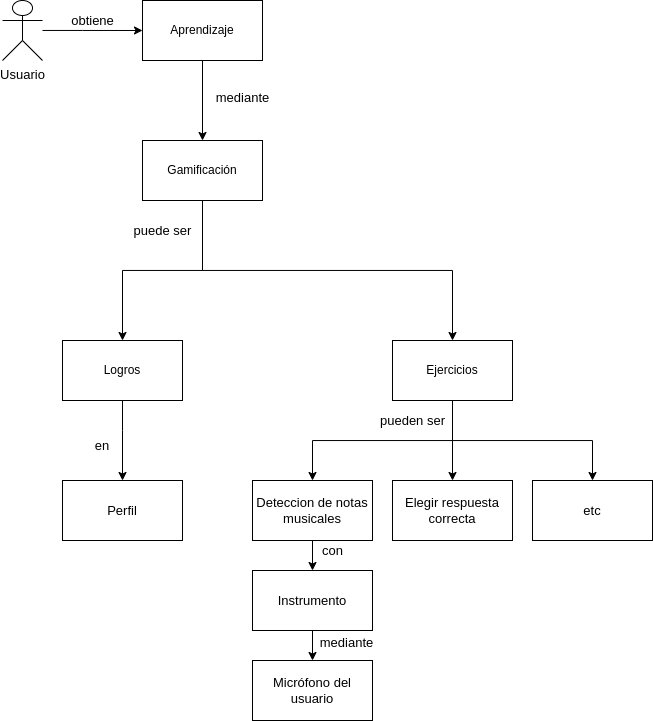
\includegraphics[width=0.8\textwidth]{imagenes/c3/diagrama.png}
    \caption{Diagrama general de la perspectiva del producto a desarrollar.}
    \label{fig:artly}

\end{figure}
Se pretende implementar un sistema que permita el aprendizaje del usuario mediante técnicas de gamificación y ejercicios a resolver. Algunas de estas actividades utilizarán librerías para la detección de notas musicales
a partir de la frecuencia captada por el micrófono del usuario y, por tanto, la aplicación dependerá de dichas librerías que se incluyan.
Por otro lado, el sistema de administración y el progreso de los usuarios se llevará a cabo utilizando una base de datos en la que se almacenará la información necesaria de los usuarios y su progreso (con un sistema de logros asociados al perfil).


La interacción de los usuarios con la aplicación será mediante una interfaz gráfica que podrá ser utilizada con la pantalla táctil o el ratón del dispositivo usado.


\subsection{Funciones del producto}
Las principales funciones que el usuario podrá realizar dentro de la aplicación son:
\begin{itemize}
\item Selección de lecciones a aprender.
\item Respuesta (mediante selección o escritura) de las preguntas y actividades que ofrezca la aplicación.
\item Consulta del progreso individual y de los logros obtenidos.
\item Modificación de los datos del perfil.
\end {itemize}

Además, el encargado/profesor se encargará de parte de la administración de las lecciones mediante:
\begin{itemize}
    \item Modificación y creación del texto de cada lección
    \item Gestión de contenido multimedia de cada lección (modificación, creación y eliminación)
    \item Gestión de las preguntas y actividades (modificación, creación y eliminación)
    \item Creación de nuevas lecciones
    \item Eliminación de lecciones
\end{itemize}

Por último, el administrador, además de las funcionalidades del encargado/profesor, podrá realizar las siguientes funcionalidades
\begin{itemize}
    \item Creación de nuevos usuarios
    \item Modificación de los datos de los usuarios
    \item Borrado de usuarios
    \item Creación de nuevas lecciones
    \item Borrado de lecciones
    \item Creación de nuevos logros
    \item Modificación de los datos de los logros
    \item Borrado de logros
\end{itemize}

\subsection{Características de los usuarios}
Los usuarios que usarán la aplicación tendrán distintos perfiles y abarcarán edades muy distintas. Aún así,
el perfil objetivo para el uso del sistema será las personas jóvenes, pues suelen utilizar mucho más las nuevas tecnologías
y estarán más familiarizados con este tipo de aplicaciones. No se necesita conocimiento musical previo para utilizar el software y,
de hecho, las lecciones pueden ser bastante básicas y sencillas para las personas que ya conozcan conceptos y aspectos avanzados del lenguaje musical.


\subsection{Restricciones}

Las restricciones del sistema a desarrollar son:
\begin{itemize}
    \item La aplicación del cliente estará desarrollada en Flutter y/o Dart y para la del servidor se utilizará NodeJS con Express.
    \item Se utilizarán las consultas, inserciones, modificaciones y borrados de MongoDB para la base de datos, usando un modelo no relacional.
    \item Al hacer uso de librerías externas para desarrollar algunas de las funciones, el rendimiento y las limitaciones hardware pueden depender de estas.
\end{itemize}


Además, es posible que el sistema tenga que adaptarse a los cambios del entorno y necesite agregar con el paso del tiempo funcionalidades que añadan valor
al producto.


\subsection{Suposiciones y dependencias}
Los requisitos especificados en este capítulo pueden estar sujetos a cambios por motivos técnicos, de alcance o de refinamiento por la necesidad de la adaptación
al entorno y a la evolución continua del proyecto.

No habrá ningúna suposición respecto al sistema operativo a utilizar puesto que pretendemos desarrollar una aplicación multiplataforma, aunque se priorizará el buen funcionamiento en Android y en navegadores web.

Asumiremos también que las bibliotecas a utilizar para el desarrollo de ciertos requisitos funcionan correctamente y son estables.

\section{Requisitos Específicos}
A continuación se listarán todos los requisitos que debe cumplir el sistema a desarrollar. Se dividirán en distintos tipos en función de sus objetivos.

\subsection{Interfaz de usuario}
Se tratará que la interfaz de usuario siga un diseño minimalista y sencillo para facilitar el uso de la aplicación a todo tipo de personas y 
garantizar cierto grado de accesibilidad. En cuanto a los colores, se usarán tonalidades de azul junto con grises.
En móviles la pantalla estará dividida en dos partes principales: 
\begin{itemize}
    \item La cabecera con el título de la aplicación, un menú estilo hamburguesa que se abrirá lateralmente y un icono para el acceso al perfil del usuario.
    \item El cuerpo, donde se encuentra el contenido principal de la sección correspondiente.
\end{itemize}

    A continuación se presenta un primer boceto de lo que podría ser la interfaz de usuario para móviles.

\begin{figure}[H]

    \centering
    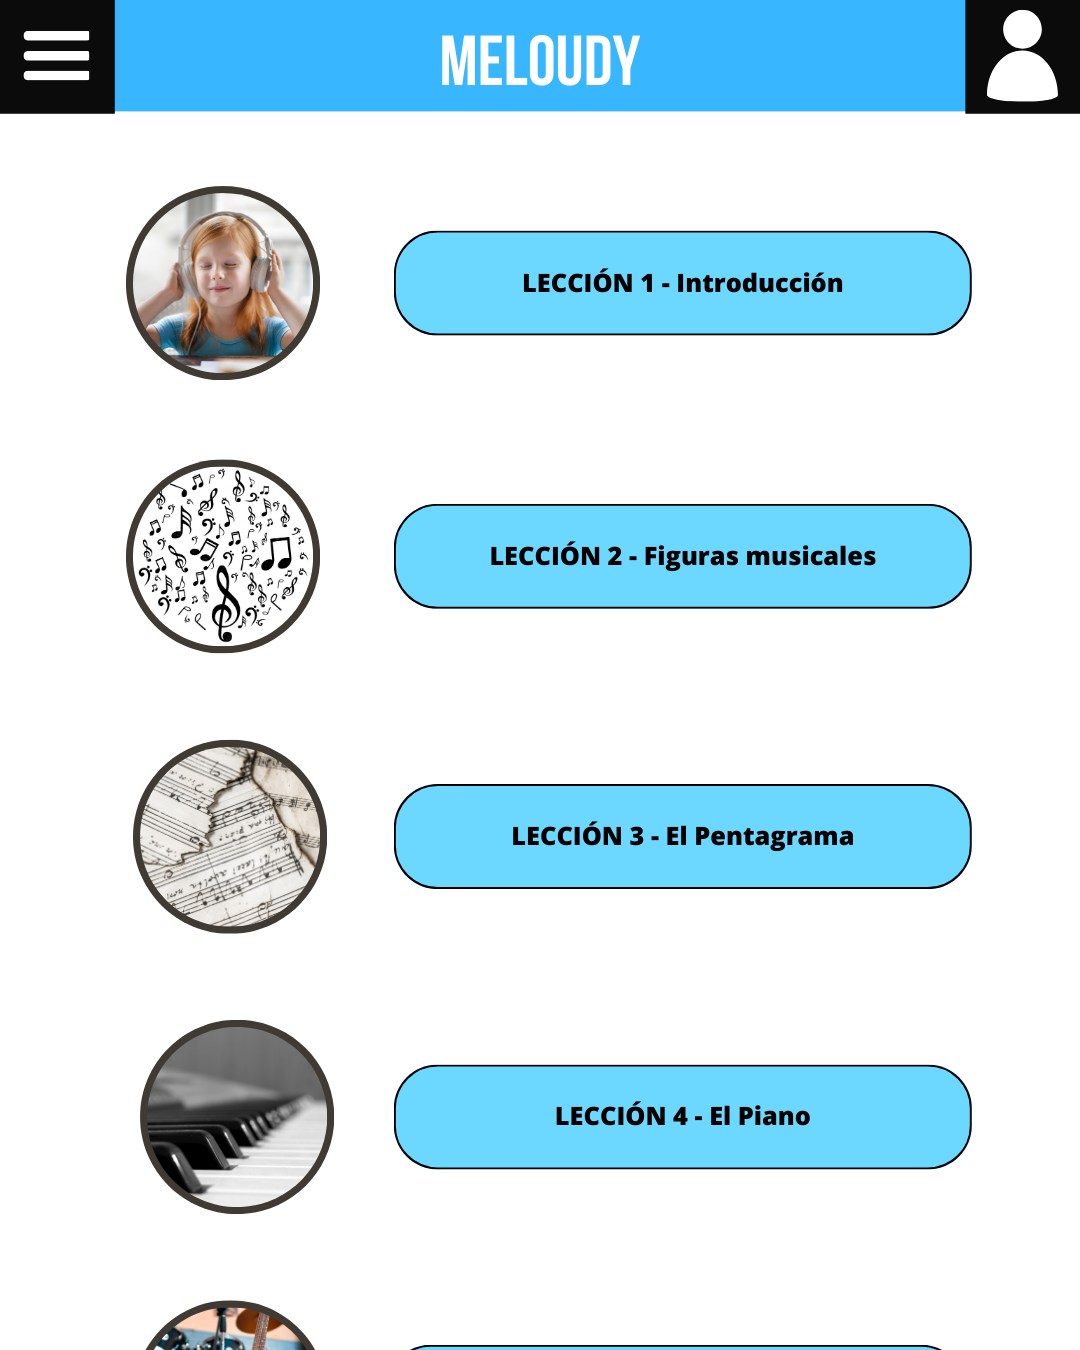
\includegraphics[width=0.7\textwidth]{imagenes/c3/boceto.png}
    \caption{Primer boceto de la interfaz de usuario de la página de inicio de la aplicación para los usuarios, donde se muestra la lista de las lecciones}
    \label{fig:artly}

\end{figure}

\subsection{Requisitos funcionales}
En esta sección se presentan los requisitos relacionados con las funcionalidades del sistema y su comportamiento, sus servicios y las tareas que este debe realizar.

\begin{itemize}
    \item \textbf{General}
          \begin{itemize}
              \item \textbf{RF 1 - Registro de usuarios: }Los usuarios deberán registrarse en el sistema para utilizar la funcionalidad de la aplicación.
              \item \textbf{RF 2 - Identificar usuarios: }Los usuarios deberán identificarse en el sistema con su cuenta para poder utilizar la funcionalidad de la aplicación.

          \end{itemize}
    \item \textbf{Usuarios}
          \begin{itemize}
              \item \textbf{RF 3 - Consultar datos del perfil: }Los usuarios podrán consultar los datos de su perfil.
              \item \textbf{RF 4 - Modificar datos del perfil: }Los usuarios podrán modificar los datos de su perfil (imagen de perfil, nombre, contraseña...).
              \item \textbf{RF 5 - Selección de lección: }Los usuarios podrán seleccionar la lección a estudiar de la lista de lecciones de la pantalla principal.
              \item \textbf{RF 6 - Responder preguntas: }Los usuarios podrán responder las preguntas de cada tipo en la lección que estén.
                    \begin{itemize}
                        \item \textbf{RF 6.1 - Responder con texto: }Los usuarios podrán responder preguntas que necesiten insertar texto como respuesta.
                        \item \textbf{RF 6.2 - Responder seleccionando varias opciones: }Los usuarios podrán responder preguntas que necesiten seleccionar varias opciones de un conjunto.
                        \item \textbf{RF 6.3 - Responder seleccionando una opción: }Los usuarios podrán responder preguntas que necesiten seleccionar una opción de un conjunto.
                        \item \textbf{RF 6.4 - Responder tocando una nota: }Los usuarios podrán responder preguntas que necesiten tocar una nota de un instrumento y captarla por el micrófono.
                    \end{itemize}º
              \item \textbf{RF 7 - Ver información de logro: }Los usuarios podrán consultar la información de un logro
              \item \textbf{RF 8 - Consultar logros del usuario: } Los usuarios podrán consultar los logros obtenidos en su perfil.
              \item \textbf{RF 9 - Consultar historial de tests: } Los usuarios podrán visualizar la lista de tests realizados de una lección en concreto.
              \item \textbf{RF 27 - Revisar test}: Los usuarios podrán revisar las respuestas de un test realizado. 
              \item \textbf{RF 22 - Consultar progreso de lección: } Los usuarios podrán consultar el progreso de una lección en concreto.
            \end{itemize}
    \item \textbf{Profesores/Encargados}
          \begin{itemize}
              \item \textbf{RF 10 - Obtener lista de lecciones: } Los profesores podrán obtener una lista de todas las lecciones que existen en el sistema.
              \item \textbf{RF 11 - Crear lección: }Los profesores podrán crear nuevas lecciones.
              \item \textbf{RF 12 - Eliminar lección: }Los profesores podrán eliminar lecciones ya existentes.
              \item \textbf{RF 13 - Modificar lecciones: }Los profesores podrán modificar el texto y el contenido multimedia de las distintas lecciones.
              \item \textbf{RF 14 - Crear preguntas: } Los profesores podrán crear nuevas preguntas sobre las distintas lecciones.
              \item \textbf{RF 15 - Obtener lista de preguntas: } Los profesores podrán obtener una lista de todas las preguntas que existen en el sistema.
              \item \textbf{RF 16 - Modificar preguntas: } Los profesores podrán modificar preguntas ya creadas.
              \item \textbf{RF 17 - Eliminar preguntas: } Los profesores podrán eliminar preguntas del sistema.
          \end{itemize}
    \item \textbf{Administradores}
          \begin{itemize}
              \item \textbf{RF 18 - Modificar datos de usuarios: }Los administradores podrán modificar los datos de un usuario.
              \item \textbf{RF 19 - Crear usuario: }Los administradores podrán crear usuarios en el sistema.
              \item \textbf{RF 20 - Obtener lista de usuarios: } Los administradores podrán obtener una lista con todos los usuarios registrados en el sistema.
              \item \textbf{RF 21 - Eliminar usuario: }Los administradores podrán eliminar usuarios registrados en el sistema.
              \item \textbf{RF 23 - Modificar datos de logro: }Los administradores podrán modificar los datos de un usuario.
              \item \textbf{RF 24 - Crear logro: }Los administradores podrán crear usuarios en el sistema.
              \item \textbf{RF 25 - Obtener lista de logros: } Los administradores podrán obtener una lista con todos los usuarios registrados en el sistema.
              \item \textbf{RF 26 - Eliminar logro: }Los administradores podrán eliminar usuarios registrados en el sistema.
          \end{itemize}
\end{itemize}

\subsection{Requisitos no funcionales}
Estos requisitos se refieren a aquellas condiciones que debe cumplir el sistema en cuanto a rendimiento, accesibilidad, seguridad, robustez...
\begin{itemize}
    \item \textbf{RNF 1 - } La aplicación cifrará las claves en todo momento para garantizar la seguridad de los usuarios.
    \item \textbf{RNF 2 - } El número de usuarios simultáneos solo estará limitado por la capacidad del hardware del servidor.
    \item \textbf{RNF 3 - } La cantidad máxima de datos a almacenar solo estará limitada por la capacidad del hardware del servidor de la base de datos.
    \item \textbf{RNF 4 - } La aplicación será multiplataforma, pudiendose ejecutar en dispositivos (móvil, ordenador, tablet...) diferentes con distintos sistemas operativos (Windows, Android...)
    \item \textbf{RNF 5 - } La aplicación será lo más accesible posible para personas con distintas discapacidades. 
    \item \textbf{RNF 6 - } La aplicación será tolerante a fallos (será fiable).
    \item \textbf{RNF 7 - } Se garantizará el cumplimiento de la Ley de Protección de Datos de Carácter Personal.
\end{itemize}



